\documentclass{article}

\usepackage[letterpaper, portrait, margin=1.5in]{geometry}

\usepackage{fancyhdr}
\usepackage{ragged2e}
\usepackage{graphicx}
\usepackage{caption}
\usepackage{amsmath}
\usepackage{rotating}
\usepackage{mwe}

\usepackage{listings}
\usepackage{color}
\usepackage{caption}
\usepackage{subcaption}

\definecolor{dkgreen}{rgb}{0,0.6,0}
\definecolor{gray}{rgb}{0.5,0.5,0.5}
\definecolor{mauve}{rgb}{0.58,0,0.82}

\lstset{frame=tb,
  language=Java,
  aboveskip=3mm,
  belowskip=3mm,
  showstringspaces=false,
  columns=flexible,
  basicstyle={\small\ttfamily},
  numbers=none,
  numberstyle=\tiny\color{gray},
  keywordstyle=\color{blue},
  commentstyle=\color{dkgreen},
  stringstyle=\color{mauve},
  breaklines=true,
  breakatwhitespace=true,
  tabsize=4
}

\setcounter{secnumdepth}{1}

\usepackage{chngcntr}
\counterwithin{figure}{section}

\renewcommand*{\thepage}{C\arabic{page}}

\pagestyle{fancy}
\lhead{ACME Robotics}
\chead{\#8367}
\rhead{\ifcontents Contents \else Week \thesection \fi}

\newif\ifcontents
\contentstrue

\makeatletter
\renewcommand{\@seccntformat}[1]{}
\makeatother
\begin{document}
\subsection{Investigate Intake Whips}
%! Investigate different types of material for the whips to improve the speed and reliability and speed of the intake.
After the Napa tournament one evident problem was that the intake was to slow. One way the team thought that this could be fixed is if the stiffness of the whips was increased. Aidan and Ashlin were designated the task of investigating different whip materials. They wanted a material that was stiff enough that it could easily hit the balls and cubes up and through the intake, but they didn't want it to be too stiff that it would cause damage to the poly carbonate shield. Aidan went to the hardware store and bought a couple different types of gas tubing of varying stiffness. The team then tested the whips and determined that to maximize the intake the thicker whips should be put with three in the middle roller as shown in figure \ref{fig:whips} and on the outer four whips for the crater roller. Aidan also determined that if he placed the most outside whips 30 degrees ahead of the rest this would help directing the balls and cubes into the center of the whips.

\begin{figure}
    \centering
    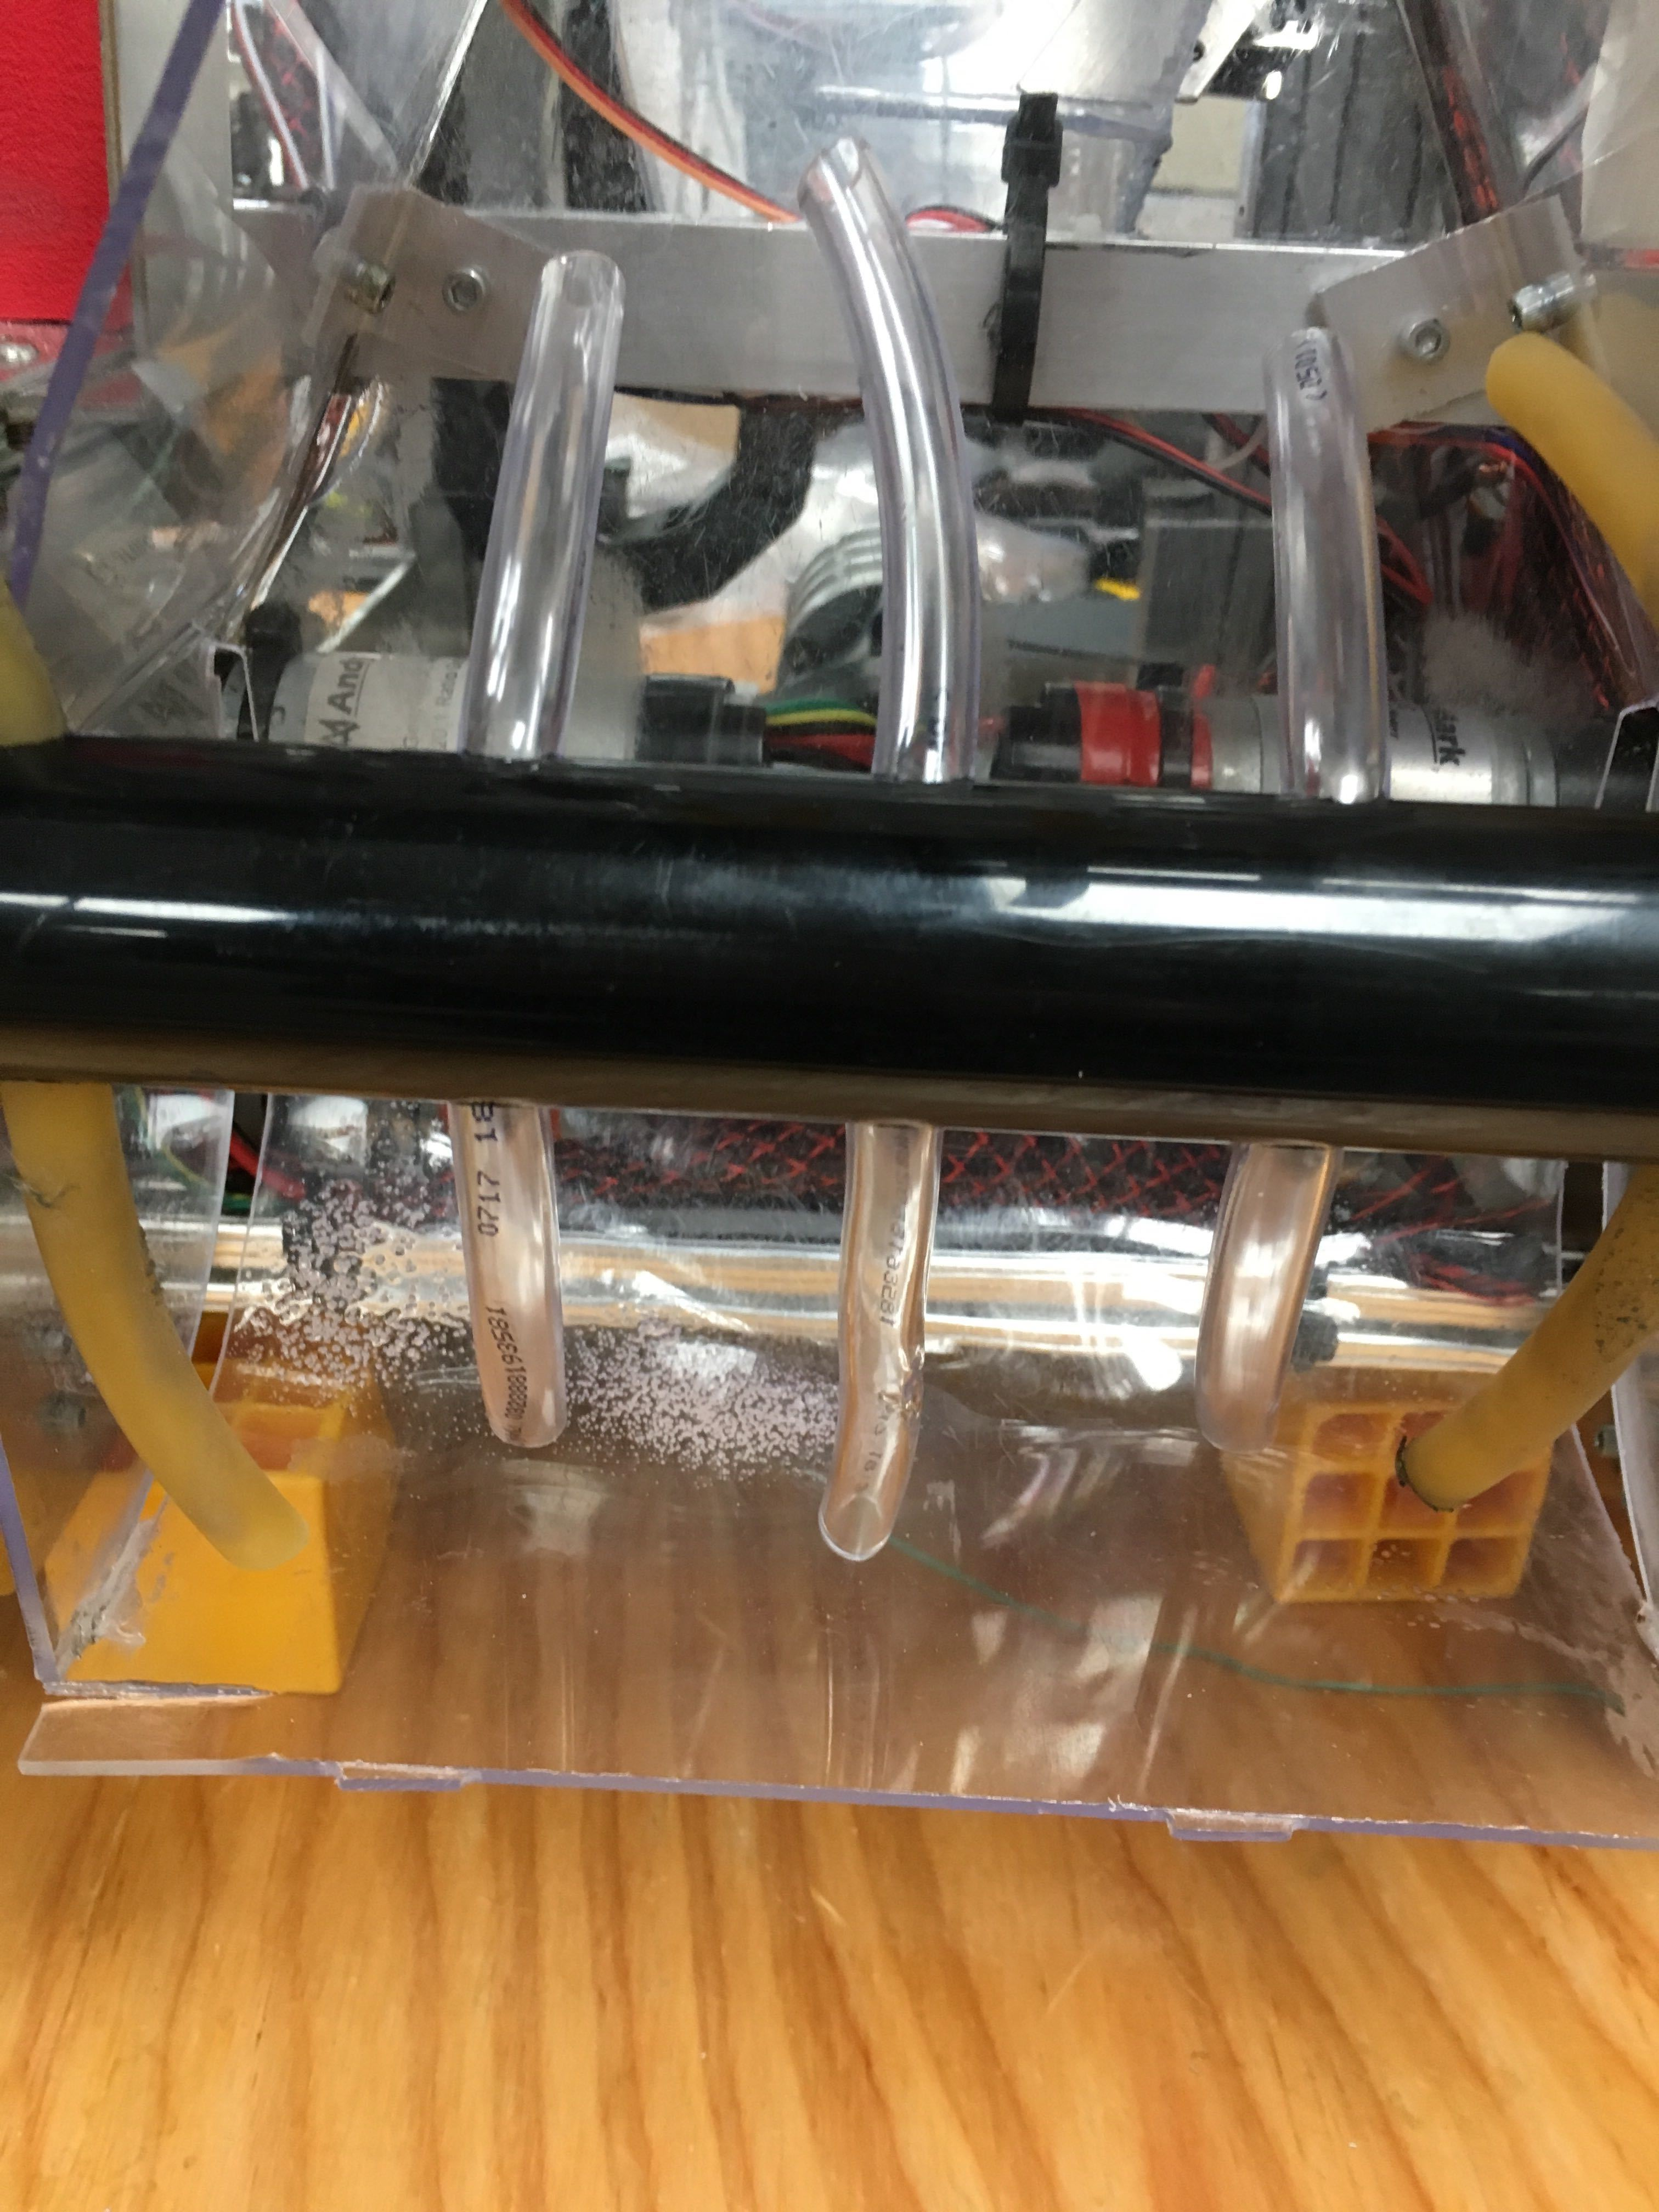
\includegraphics[width=.6 \textwidth]{24_02-11/images/intakewhips.JPG}
    \caption{Intake Whips}
    \label{fig:whips}
\end{figure}

\subsection{Lift Version 2.0}
%! Create a new lift design to fix problems with the current design including height inconsistency and sloppy tolerances.
After the Napa tournament, it was evident that there was some issues and restrictions with the current design of the lift. The most notable ones being the inconstant lift height through out a match, and the over all lack of tolerances due to the bearing blocks assembling process. With both of these issues so closely affecting the over all performance, the hardware team set out with two plans to fix the problems. Oren set out re-CADing, and ordering new parts for a second lift, that would be able to easily be switched out for the current one when the time came. Meanwhile the other hardware members made parts and improvements to the current lift as a precaution in case the new lift wasn't made in time for NorCals. 


\subsection{Change the Lift String Standoffs}
%! Fabricate custom lift string standoffs to eliminate problems resulting from standoffs bending.
One recurring problem that was noticed prior and during the Napa tournament was that the pull up run length was very inconsistent. This was because the standoffs that held the pull up run bearings continued to bend which changed the overall length. Aidan was designated the task of creating more reliable standoffs. He decided that the best way to do this would be to manufacture custom pieces for each bearing location. He completed CAD drawing of each desired piece as shown in figure \ref{fig:PullUp1} and \ref{fig:PullUp2} and planned to cut the parts out the next week.

\begin{figure}[h!]
\centering
\begin{subfigure}{.45\textwidth}
  \centering
  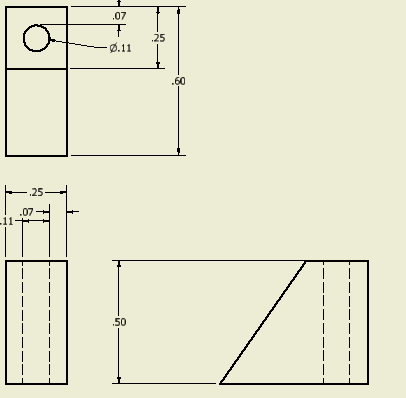
\includegraphics[height=3.5cm]{24_02-11/images/PullUpBlock1.PNG}
    \caption{Pull Up Block 1}
    \label{fig:PullUp1}
 \end{subfigure}
\begin{subfigure}{.45\textwidth}
  \centering
     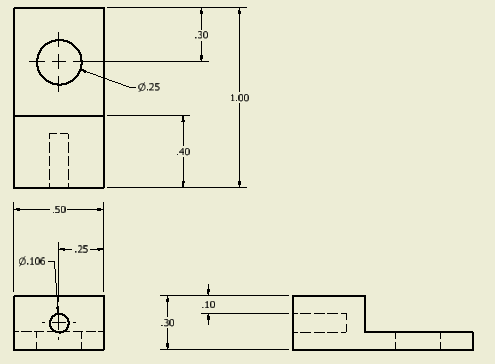
\includegraphics[height=3.5cm]{24_02-11/images/PullUp2.PNG}
    \caption{Pull Up Block 2}
    \label{fig:PullUp2}
  \end{subfigure}
  \caption{Drivetrain components}
  \end{figure}



\end{document} 